%%-*-latex-*-

% ------------------------------------------------------------------------
%
\begin{frame}
\frametitle{Stacks}

Let us specify now a linear data structure, called \textbf{stack}.

\bigskip

A stack is similar to a pile of paper sheets on a table: we can only
add a new sheet on its top (this is called \textbf{to push}) and
remove one on its top (this is called \textbf{to pop}).

\bigskip

From this informal description, we understand that we shall need a
constructor for the stack that takes an argument (like a sheet): it is
a function. This is different from the boolean constructors which are
constants (\proc{True} and \proc{False}).

\end{frame}

% ------------------------------------------------------------------------
%
\begin{frame}
\frametitle{Stacks (cont)}

How do we model the fact that the stack has changed after a pop or a
push? The simplest is to imagine that we give the original stack as an
argument and the function calls (pop/push) represent the modified
stack.

\bigskip

Also, we do not want to specify actually the nature of the elements in
the stack, in order to be general: we need a parameter type for the
elements.

\end{frame}

% ------------------------------------------------------------------------
%
\begin{frame}
\frametitle{Stacks/Signature}

Let us call \(\proc{Stack} (\type{item})\) the specification of
a stack over the \type{item} type.
\begin{itemize}

  \item \textbf{Parameter types}

  \begin{itemize}

    \item The type \type{item} of the elements in the stack.

  \end{itemize}

  \item \textbf{Defined types}

   \begin{itemize}

     \item The type of the stacks is \type{t}.

   \end{itemize}

  \item \textbf{Constructors}

  \begin{itemize}

    \item \(\proc{Empty} : \type{t}\)\\
    Expression \proc{Empty} represents the empty stack.

    \item \(\proc{Push} : \type{item} \times \type{t}
    \rightarrow \type{t}\)\\
    Expression \(\proc{Push} (\id{e}, \id{s})\) denotes the stack
    \id{s} with element \id{e} pushed on top.

  \end{itemize}

\end{itemize}

\end{frame}

% ------------------------------------------------------------------------
%
\begin{frame}
\frametitle{Stacks/Constructors}

We need a \textbf{constant constructor} to stand for the empty stack,
otherwise we would not know what stack remains after popping a stack
containing only one element.

\bigskip

The type of \proc{Push} is \(\type{item} \times \type{t}
\rightarrow \type{t}\), which means it is a \textbf{non-constant
constructor} (it is a special case of function, basically) which takes
a pair made of an element and a stack and returns a new stack (with
the element on top).

\bigskip

Here are some stacks:
\begin{itemize}

  \item \proc{Empty}

  \item \(\proc{Push} (\id{e_1}, \proc{Push} (\id{e_2}, \proc{Empty}))\)

\end{itemize}

\end{frame}

% ------------------------------------------------------------------------
%
\begin{frame}
\frametitle{Stacks/Projections}

We can complement this definition with other functions which allows us
to extract information from a given stack. In particular, a function
which gives us back the information which was given to some
constructor is called a \textbf{projection}. \emph{A projection is the
inverse function of a constructor.}

\bigskip

The constant constructor \proc{Empty} has no inverse function, because
it can be considered as equivalent to a function \(f\) defined as
\(\forall \id{x}.f (\id{x}) = \proc{Empty}\), whose inverse \(f^{-1}\)
is not a function because it maps \proc{Empty} to any \id{x}.

\bigskip

Thus we only care of \textbf{non-constant constructors}, i.e., the ones
which take arguments.

\end{frame}

% ------------------------------------------------------------------------
%
\begin{frame}
\frametitle{Stacks/Projections and other functions}

Since the specification \(\proc{Stack}(\type{item})\) has only one
non-constant constructor, we have only one projection. We can also add
a function \proc{Append}.

\bigskip

Here is how the signature continues:
\begin{itemize}

  \item \textbf{Projections}

  \begin{itemize}

    \item \(\proc{Pop} : \type{t} \rightarrow \type{item} \times
      \type{t}\)\\ This projection is the inverse of constructor
      \proc{Push}.

  \end{itemize}

  \item \textbf{Other functions}

  \begin{itemize}

    \item \(\proc{Append} : \type{t} \times \type{t} \rightarrow
      \type{t}\)\\ Expression \(\proc{Append} (\id{s_1}, \id{s_2})\)
      represents a stack made of stack \id{s_1} on top of stack
      \id{s_2}.

  \end{itemize}

\end{itemize}

\end{frame}

% ------------------------------------------------------------------------
%
\begin{frame}
\frametitle{Stacks/Equations}

Now the defining equations of the stack:
{\small
\begin{align*}
\proc{Pop}  \circ \proc{Push} &= \id{id}\\
\proc{Append} (\proc{Empty}, \proc{Empty}) &= \proc{Empty}\\
  \proc{Append} (\proc{Empty}, \proc{Push} (e, s)) 
   &= \proc{Push} (e, s)\\
\proc{Append} (\proc{Push} (e, s), \proc{Empty}) 
   &= \proc{Push} (e, s)\\
\proc{Append} (\proc{Push} (e_1, s_1), \proc{Push}
     (e_2, s_2))
   &= \proc{Push} (e_1, \proc{Append} (s_1, \proc{Push} (e_2, s_2)))
\end{align*}
}
where \(\overline{e} = (e_1, e_2)\),
\(\overline{s} = (s_1, s_2)\) and \id{id} is the
identity function \(\forall x.x \mapsto x\).

\end{frame}

% ------------------------------------------------------------------------
%
\begin{frame}
\frametitle{Stacks/Prefixing}

If we refer to the type of stacks over elements of type
\type{item} \emph{outside its definition}, we have to write:
\[\proc{Stack} (\type{item}).\type{t}\]

\bigskip

So the empty stack is noted \(\proc{Stack}
(\type{item}).\proc{Empty}\) outside the \proc{Stack} specification,
in order to avoid confusion with
\proc{Bin-tree}.(\type{node}).\proc{Empty}, for instance.

\bigskip

If the context is not ambiguous, e.g., we know that we are talking
about stacks, we can omit the prefix ``\proc{Stack}.'' and simply
write \proc{Empty}, for instance.

\end{frame}

% ------------------------------------------------------------------------
%
\begin{frame}
\frametitle{Stacks/Recursive equations}
\label{sequence}

An interesting point in the previous equations is that the function
\proc{Append} is defined on terms of itself. This kind of equation is
called \textbf{recursive}.

\bigskip

This is not new for you. In high school you became familiar with
\textbf{integer sequences} defined by equations like
\[\begin{aligned}
    U_{n+1} &= b + U_{n}\\
    U_{0} &= a
  \end{aligned}
\]
This is exactly equivalent to
\[\begin{aligned}
    U(n+1) &= b + U(n)\\
    U(0) &= a
  \end{aligned}
\]
Only the notation differs. The meaning is the same.

\end{frame}

% ------------------------------------------------------------------------
%
\begin{frame}
\frametitle{Stacks/Simplifying the equations}

We can ease the notation by omitting the quantifiers \(\forall\) in
equations. Also, we can simplify a little the equations for
\proc{Append} by noting that if one of the stack is empty, then the
result is always the other stack:
\[
\left\{
\begin{aligned}
   \proc{Append} (\proc{Empty}, \proc{Empty}) 
&= \proc{Empty}\\
   \forall e, s \quad \proc{Append} (\proc{Empty},
   \proc{Push} (e, s)) 
&= \proc{Push} (e, s)\\
   \forall e, s \quad \proc{Append} (\proc{Push}
   (e, s), \proc{Empty}) 
&= \proc{Push} (e, s)
\end{aligned}
\right.
\]
\[
\stackrel{?}{\Longleftrightarrow}
\left\{
\begin{aligned}
\proc{Append} (\proc{Empty}, s) &= s\\
\proc{Append} (s, \proc{Empty}) &= s
\end{aligned}
\right.
\]

\end{frame}

% ------------------------------------------------------------------------
%
\begin{frame}
\frametitle{Stacks/Simplifying the equations (cont)}

The way to check this is to note that there are only two kinds of
stacks, empty and no-empty, so we can replace \id{s} respectively by
\proc{Empty} and \(\proc{Push} (\id{e}, \id{s})\) in the new system:
\[\footnotesize
\left\{
\begin{aligned}
\proc{Append} (\proc{Empty}, \id{s}) &= \id{s}\\
\proc{Append} (\id{s}, \proc{Empty}) &= \id{s}
\end{aligned}
\right.
\Leftrightarrow
\left\{
\begin{aligned}
\proc{Append} (\proc{Empty}, \proc{Empty}) &= \proc{Empty}\\
\proc{Append} (\proc{Empty}, \proc{Push} (\id{e}, \id{s})) &=
\proc{Push} (\id{e}, \id{s})\\
\proc{Append} (\proc{Empty}, \proc{Empty}) &= \proc{Empty}\\
\proc{Append} (\proc{Push} (\id{e}, \id{s}), \proc{Empty}) &=
\proc{Push} (\id{e}, \id{s})
\end{aligned}
\right.
\]
The first and third equations are the same. The system is the same as
the original one.
\end{frame}

% ------------------------------------------------------------------------
%
\begin{frame}
\frametitle{Stacks/Orienting the equations}

Let us call \textbf{term} the objects constructed using the functions
of the specification, e.g., \proc{Empty} and \(\proc{Push} (\id{e},
\proc{Empty})\) are terms. The \(e\) in the latter term is called a
\textbf{variable} (and is a special case of term).

\bigskip

We call \textbf{subterm} a term embedded in a term. For instance
\begin{itemize}

  \item \proc{Empty} is a subterm of \(\proc{Push} (\id{e},
  \proc{Empty})\);

  \item \(\proc{Push} (\id{e_1}, \proc{Empty})\) is a subterm of
  \(\proc{Push} (\id{e_2}, \proc{Push} (\id{e_1}, \proc{Empty}))\);

  \item \id{e} is a subterm of \(\proc{Push} (\id{e},
  \proc{Empty})\);

  \item \id{e} is a subterm of \id{e} (it is not a \emph{proper}
  subterm, though).

\end{itemize}

\end{frame}

% ------------------------------------------------------------------------
%
\begin{frame}
\frametitle{Stacks/Orienting the equations (cont)}

How do we orient
\begin{align*}
   \proc{Pop} (\proc{Push} (\id{x}))
&= \id{x}\\
   \proc{Append} (\proc{Empty}, \id{s}) 
&= \id{s}\\
   \proc{Append} (\id{s}, \proc{Empty}) 
&= \id{s}\\
   \proc{Append} (\proc{Push} (\id{e}, \id{s_1}), \id{s_2}) 
&= \proc{Push} (\id{e}, \proc{Append} (\id{s_1}, \id{s_2}))
\end{align*}

\end{frame}

% ------------------------------------------------------------------------
%
\begin{frame}
\frametitle{Stacks/Orienting the equations (cont)} 

The first three ones are easy to orient since no function call of the
defined function appear on both sides:
\begin{align*}
   \proc{Pop} (\proc{Push} (\id{x}))
&\rightarrow \id{x}\\
   \proc{Append} (\proc{Empty}, \id{s}) 
&\rightarrow_1 \id{s}\\
   \proc{Append} (\id{s}, \proc{Empty}) 
&\rightarrow_2 \id{s}\\
   \proc{Append} (\proc{Push} (\id{e}, \id{s_1}), \id{s_2}) 
&= \proc{Push} (\id{e}, \proc{Append} (\id{s_1}, \id{s_2}))
\end{align*}
The last equation is a recursive equation, i.e., there is a function
call of the defined function on both side of the equality. How should
we orient it?

\end{frame}

% ------------------------------------------------------------------------
%
\begin{frame}
\frametitle{Stacks/Orienting the equations (cont)} 

Let us colour both calls to \proc{Append}:
\[
\textbf{\proc{Append} (\proc{Push} (\id{e}, \id{s_1}), \id{s_2})}
= \proc{Push} (\id{e}, \textbf{\proc{Append} (\id{s_1}, \id{s_2})})
\]
Let us colour only the differences between the two:
\[
\proc{Append} (\textbf{\proc{Push} (\id{e}, \id{s_1})}, \id{s_2})
= \proc{Push} (\id{e}, \proc{Append} (\textbf{\id{s_1}}, \id{s_2}))
\]
Obviously, \id{s_1} is a \emph{proper} subterm of \(\proc{Push}
(\id{e}, \id{s_1})\), so the value of \(s_1\) is included in the value
of \(\proc{Push} (\id{e}, \id{s_1})\). The call-by-value strategy
implies that the value of \(\proc{Append} (\id{s_1}, \id{s_2})\) is
included in the value of \(\proc{Append} (\proc{Push} (\id{e},
\id{s_1}), \id{s_2})\). Therefore we must orient the equation from
left to right.

\end{frame}

% ------------------------------------------------------------------------
%
\begin{frame}
\frametitle{Stacks/Orienting the equations (cont)} 

What is the use of \(\proc{Append} (\id{s}, \proc{Empty})
\rightarrow_2 \id{s}\)?

\bigskip

It is actually useless because the first argument of \proc{Append}
will always become \proc{Empty}, since we replace it by a proper
subterm at each rewriting, the second rewriting rule \(\proc{Append}
(\proc{Empty}, \id{s}) \rightarrow_1 \id{s}\) always applies at the
end. So we only need:
\begin{align*}
   \proc{Append} (\proc{Empty}, \id{s}) 
&\rightarrow \id{s}\\
   \proc{Append} (\proc{Push} (\id{e}, \id{s_1}), \id{s_2})
&\rightarrow \proc{Push} (\id{e}, \proc{Append} (\id{s_1}, \id{s_2}))
\end{align*}
The only difference is the \textbf{complexity}, that is, in this
framework of rewriting systems, the number of steps needed to reach
the result. With rule \(\rightarrow_2\), if the second stack is empty,
we can conclude in one step. Without it, we have to traverse all the
elements of the first stack before terminating.

\end{frame}

% ------------------------------------------------------------------------
%
\begin{frame}
\frametitle{Stacks/Terms as trees}

Let us find a model which clarifies these ideas: the concept of
\textbf{tree}.

\bigskip

A tree is either 
\begin{itemize}

  \item the empty set

  \item or a tuple made of a \textbf{root} and other trees, called
  \textbf{subtrees}.

\end{itemize}
This is a \textbf{recursive definition} because the object (here, the
tree) is defined by case and by grouping objects of the same kind
(here, the subtrees).

\bigskip

A root could be further refined as containing some specific
information.

\bigskip

It is usual to call \textbf{nodes} the root of a given tree and the
roots of all its subtrees, \emph{transitively}.

\bigskip

A node without non-empty subtrees is called a \textbf{leaf}.

\end{frame}

% ------------------------------------------------------------------------
%
\begin{frame}
\frametitle{Stacks/Terms as trees (cont)}

If we consider trees as relationships between nodes, it is usual to
call a root the \textbf{parent} of the roots of its direct subtrees
(i.e., the ones immediately in the tuple). Conversely, these roots are
\textbf{sons} of their parent (they are ordered).

It is also common to call subtree any tree included in it according to
the subset relationship (otherwise we speak of \emph{direct} subtrees).

Trees are often represented in a top-down way, the root being at the
top of the page, nodes as circles and the relationship between nodes
as \textbf{edges}. For instance:

\begin{center}
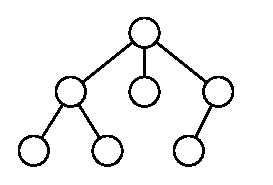
\includegraphics[bb=71 648 175 721]{tree_example}
\end{center}

\end{frame}

% ------------------------------------------------------------------------
%
\begin{frame}
\frametitle{Stacks/Terms as trees (cont)}

The \textbf{depth} of a node is the length of the path from the root
to it (note this path is unique). Thus the depth of the root is 0 and
the depth of the empty tree is undefined.

\bigskip

The \textbf{height} of a tree is the maximal depth of its nodes. For
example, the height of the tree in the previous page is 2.

\bigskip

A \textbf{level} in a tree is the set of all nodes with a given
depth. Hence it is possible to define level 0, level 1 etc. (may be
empty).

\end{frame}

% ------------------------------------------------------------------------
%
\begin{frame}
\frametitle{Stacks/Height of terms}

This leads us to consider \emph{values} as \emph{trees}
themselves. Each constructor corresponds to a node, and each argument
corresponds to a subtree. By definition:
\[
\begin{array}{c|c|c}
  \text{Term}
& \text{Tree}
& \text{Height}\\
\hline\hline
  \proc{Empty} 
& \proc{Empty}
& 0\\
\hline
  \proc{Push} (\id{e}, \id{s})
& 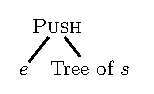
\includegraphics{push_tree}
& 1 + \text{height of tree of \id{s}}
\end{array}
\]
Now we can think the ``size'' of a value as the \textbf{height of the
corresponding tree}.

\end{frame}

% ------------------------------------------------------------------------
%
\begin{frame}
\frametitle{Stacks/Height of terms (cont)} 

Let us define a function, called \textbf{height} and written \({\cal
 H}\), for each term denoting a stack in the following way:
\[
\begin{aligned}
&                       &    {\cal H} (\proc{Empty}) 
                          &= 0\\
&\forall \id{e}, \id{s} &    {\cal H} (\proc{Push} (\id{e}, \id{s}))
                          &= {\cal H} (\id{s}) + 1
\end{aligned}
\]
where \(x\) is a variable denoting an element and \(s\) a variable
denoting a stack.

\end{frame}
